\documentclass[border=8pt]{standalone}
\usepackage[T1]{fontenc}\usepackage{lmodern}\usepackage{amsmath}\usepackage[dvipsnames]{xcolor}
\usepackage{tikz}\usetikzlibrary{positioning,arrows.meta,fit,backgrounds,calc,shapes.geometric}
% ---- colours of the system diagrams (one per MQTT topic / kind of traffic)
\definecolor{cSensor}{RGB}{37,99,235}     % sensors/<node>
\definecolor{cAlert}{RGB}{220,38,38}      % ids/alerts
\definecolor{cStats}{RGB}{22,163,74}      % ids/stats
\definecolor{cMit}{RGB}{124,58,237}       % ids/mitigation/status
\definecolor{cStatus}{RGB}{100,116,139}   % ids/status
\definecolor{cCmd}{RGB}{234,88,12}        % cmd/mitigation
\definecolor{cAttack}{RGB}{153,27,27}     % attack traffic
\definecolor{cBot}{RGB}{161,98,7}         % bot master commands (UDP, not MQTT)
\definecolor{cPi}{RGB}{220,38,90}
\definecolor{cLap}{RGB}{51,65,85}
\definecolor{cNode}{RGB}{8,145,178}
\newcommand{\topicdot}[1]{\textcolor{#1}{\rule{0.9em}{0.9em}}}

\tikzset{
  box/.style={draw=#1!70!black, fill=#1!8, rounded corners=4pt, align=center, font=\small, line width=0.7pt,
              inner sep=6pt},
  box/.default=gray,
  group/.style={draw=#1, rounded corners=8pt, line width=1.1pt, inner sep=10pt},
  grouplabel/.style={font=\bfseries\small, text=#1, fill=white, inner sep=3pt},
  pub/.style={-{Stealth[length=7pt]}, line width=1.3pt, draw=#1},
  deliver/.style={-{Stealth[length=7pt]}, line width=1.3pt, draw=#1, dashed},
  attack/.style={-{Stealth[length=8pt]}, line width=1.8pt, draw=cAttack, densely dashed},
  botcmd/.style={-{Stealth[length=7pt]}, line width=1.3pt, draw=cBot, densely dotted},
  lbl/.style={font=\scriptsize\ttfamily, text=#1, fill=white, inner sep=1.5pt},
  flow/.style={-{Stealth[length=6pt]}, line width=1pt, draw=gray!70!black},
}

\begin{document}
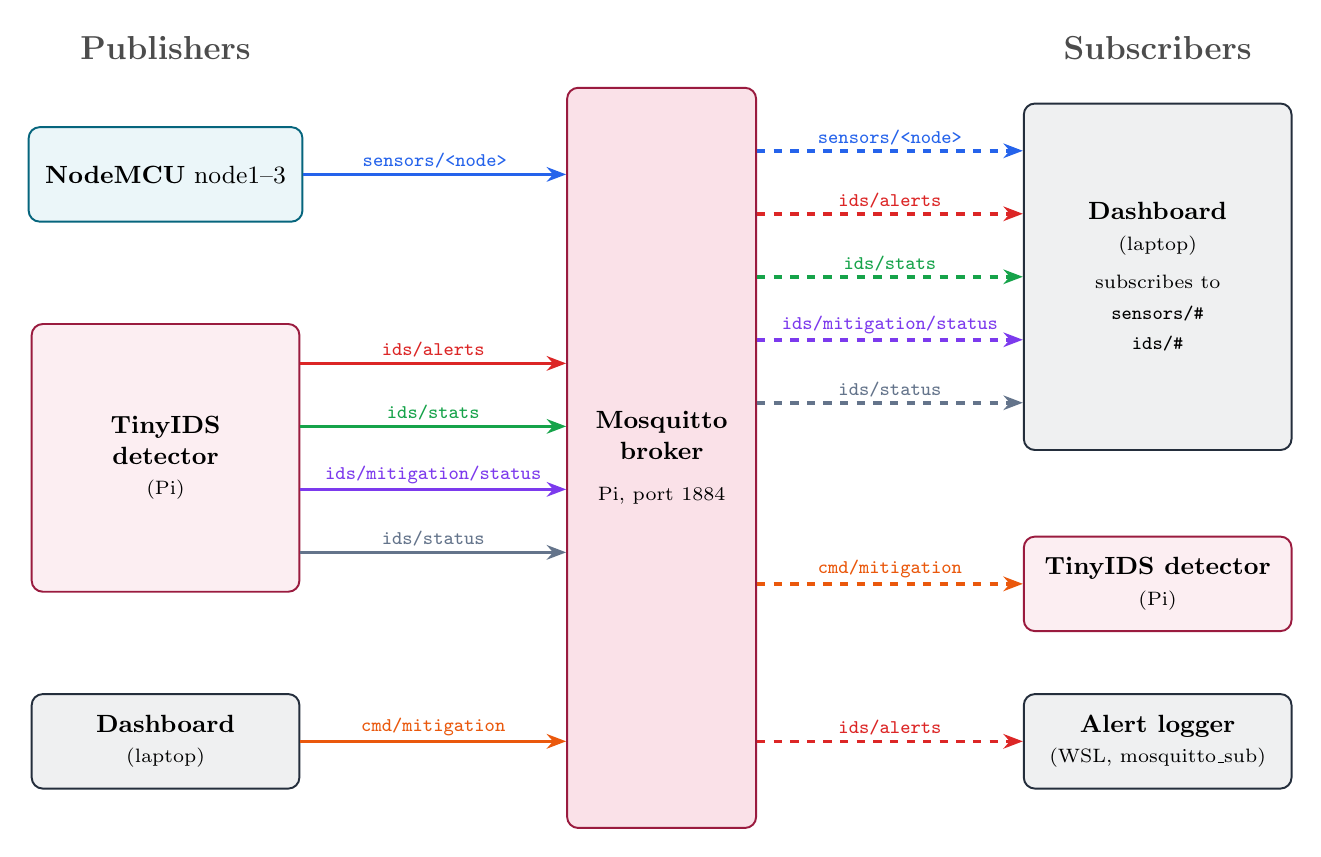
\begin{tikzpicture}[font=\small]

% publishers (left)
\node[font=\bfseries\large, text=gray!60!black] at (1.7,5.2) {Publishers};
\node[box=cNode, minimum width=3.4cm, minimum height=1.2cm] (pN) at (1.7,3.6) {\textbf{NodeMCU} node1--3};
\node[box=cPi, minimum width=3.4cm, minimum height=3.4cm] (pI) at (1.7,0) {\textbf{TinyIDS}\\\textbf{detector}\\{\scriptsize (Pi)}};
\node[box=cLap, minimum width=3.4cm, minimum height=1.2cm] (pD) at (1.7,-3.6) {\textbf{Dashboard}\\{\scriptsize (laptop)}};

% broker
\node[box=cPi, minimum width=2.4cm, minimum height=9.4cm, fill=cPi!14] (B) at (8,0)
  {\textbf{Mosquitto}\\\textbf{broker}\\[4pt]{\scriptsize Pi, port 1884}};

% subscribers (right)
\node[font=\bfseries\large, text=gray!60!black] at (14.3,5.2) {Subscribers};
\node[box=cLap, minimum width=3.4cm, minimum height=4.4cm] (sD) at (14.3,2.3) {\textbf{Dashboard}\\{\scriptsize (laptop)}\\[3pt]{\scriptsize subscribes to}\\{\scriptsize\ttfamily sensors/\#}\\{\scriptsize\ttfamily ids/\#}};
\node[box=cPi, minimum width=3.4cm, minimum height=1.2cm] (sI) at (14.3,-1.6) {\textbf{TinyIDS detector}\\{\scriptsize (Pi)}};
\node[box=cLap, minimum width=3.4cm, minimum height=1.2cm] (sL) at (14.3,-3.6) {\textbf{Alert logger}\\{\scriptsize (WSL, mosquitto\_sub)}};

% incoming (publish), solid
\draw[pub=cSensor] (pN.east) -- node[lbl=cSensor, above] {sensors/<node>} (pN.east -| B.west);
\draw[pub=cAlert]  ($(pI.east)+(0,1.2)$)  -- node[lbl=cAlert, above] {ids/alerts} ($(pI.east -| B.west)+(0,1.2)$);
\draw[pub=cStats]  ($(pI.east)+(0,0.4)$)  -- node[lbl=cStats, above] {ids/stats} ($(pI.east -| B.west)+(0,0.4)$);
\draw[pub=cMit]    ($(pI.east)+(0,-0.4)$) -- node[lbl=cMit, above] {ids/mitigation/status} ($(pI.east -| B.west)+(0,-0.4)$);
\draw[pub=cStatus] ($(pI.east)+(0,-1.2)$) -- node[lbl=cStatus, above] {ids/status} ($(pI.east -| B.west)+(0,-1.2)$);
\draw[pub=cCmd]    (pD.east) -- node[lbl=cCmd, above] {cmd/mitigation} (pD.east -| B.west);

% outgoing (deliver), dashed
\draw[deliver=cSensor] ($(B.east |- sD.east)+(0,1.6)$)  -- node[lbl=cSensor, above] {sensors/<node>} ($(sD.west)+(0,1.6)$);
\draw[deliver=cAlert]  ($(B.east |- sD.east)+(0,0.8)$)  -- node[lbl=cAlert, above] {ids/alerts} ($(sD.west)+(0,0.8)$);
\draw[deliver=cStats]  ($(B.east |- sD.east)+(0,0)$)    -- node[lbl=cStats, above] {ids/stats} ($(sD.west)+(0,0)$);
\draw[deliver=cMit]    ($(B.east |- sD.east)+(0,-0.8)$) -- node[lbl=cMit, above] {ids/mitigation/status} ($(sD.west)+(0,-0.8)$);
\draw[deliver=cStatus] ($(B.east |- sD.east)+(0,-1.6)$) -- node[lbl=cStatus, above] {ids/status} ($(sD.west)+(0,-1.6)$);
\draw[deliver=cCmd]    (B.east |- sI.west) -- node[lbl=cCmd, above] {cmd/mitigation} (sI.west);
\draw[deliver=cAlert]  (B.east |- sL.west) -- node[lbl=cAlert, above] {ids/alerts} (sL.west);

\end{tikzpicture}
\end{document}
